\documentclass[12pt]{extarticle}

\setlength{\headheight}{15pt} % ??? we do what fancyhdr tells us to do  

\title{Physics 2    }
\author{Giacomo Ellero}
\date{a.y. 2024/2025}

\usepackage{preamble}

% \renewcommand{\vec}[1]{\uvec{#1}}

\begin{document}

\firstpage

\section{Mathematical tools}

\subsection{Scalar and vector fields}

\begin{definition}{Scalar field}{scalar-field}
    A scalar field is a function of type $f:\R^d \to \R$.
\end{definition}

Some examples of scalar fields are temperature or pressure.

\begin{definition}{Level curve of a scalar field}{level-curve-scalar}
    Let $f$ be a scalar field and $k \in \R$ constant.
    Then a level curve of $f$ at $k$ is the set
    \begin{equation}
        \left\{ \vec x \in \R^d : f(\vec x) = k  \right\}
    \end{equation}
\end{definition}


\begin{definition}{Vector field}{vector-field}
    A vector field is a function of type $\vec g: \R^d \to \R^d$.
\end{definition}

Some examples of vector fields are gravitational fields or the velocity field of fluids.

We will always work with \say{well behaved} fields: this means the functions are \say{almost always infinite} (of class $C^\infty$ with only some points as exceptions).

\begin{example}{}{vec-field}
    Let $\vec g(x, y, z) = x \hat x + y \hat y + z \hat z$.

    \begin{figure}[H]
        \centering
        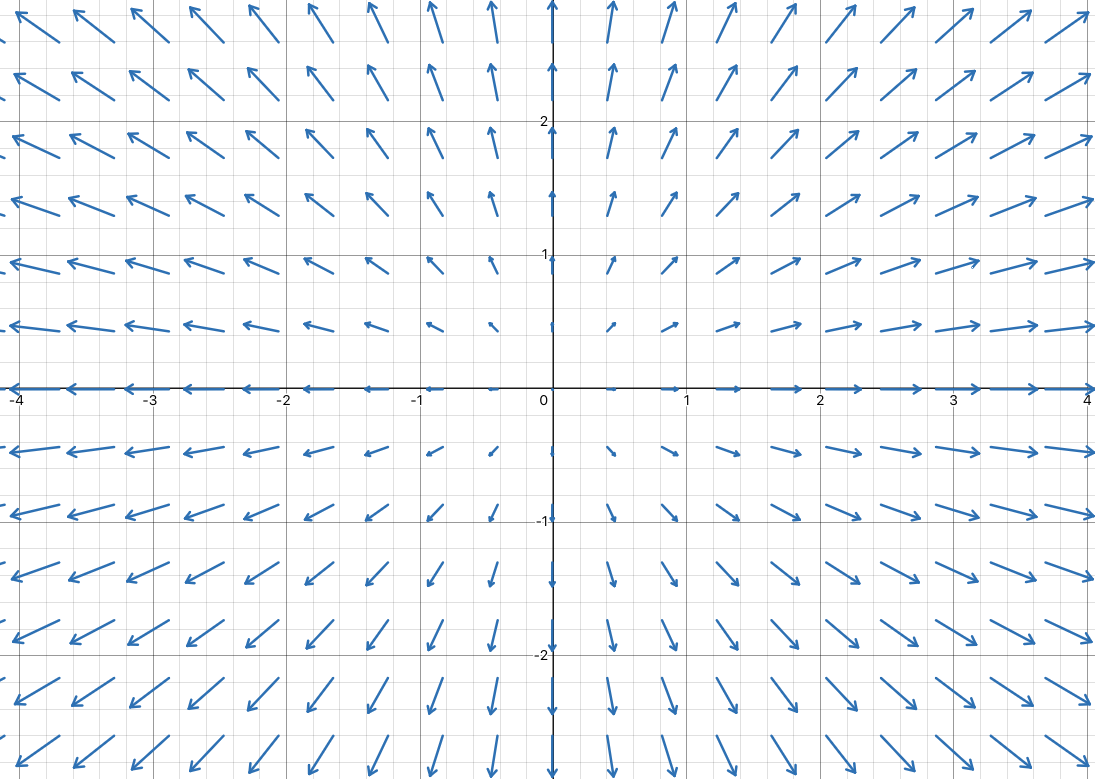
\includegraphics[width=0.6\textwidth]{assets/physics-2/vector-field-example.png}
        \caption{The arrow representation of $\vec g$ when $z = 0$.}
    \end{figure}
\end{example}

Some vector fields have \say{special points} where there are an infinite number of field lines going through it:
\begin{itemize}
    \item If all the lines go into that point we call such point \textbf{source} (the point $(0,0,0)$ is a source for \Cref{ex:vec-field});
    \item If all the lines go out of that point we call such point \textbf{sink} (use the field $\vec g(x, y, z) = -x \hat x - y \hat y - z \hat z$ as an example).
\end{itemize}
It is possible for some vector fields to have no sources or sinks. Some patterns that can arise are \textit{loops} or \textit{straight lines}.

\subsection{Operations over fields}

\begin{definition}{Gradient of a scalar field}{gradient-scalar}
    We define the gradient as
    \begin{equation}
        \vec \nabla f = \pdv{f}{x} \hat{x} + \pdv{f}{y} \hat{y} + \pdv{f}{z} \hat{z}
    \end{equation}

    We can also define the differential of a field as follows (where $\dd{l} = \dd{x} \hat{x} + \dd{y} \hat{y} + \dd{z} \hat{z} $):
    \begin{equation}
        \dd{f} = \pdv{f}{x} \dd{x} + \pdv{f}{y} \dd{y} + \pdv{f}{z} \dd{z} = \vec \nabla f \cdot \dd{\vec l}
    \end{equation}
\end{definition}

The gradient of a field is somewhat the equivalent of the derivative for 1D functions.

\begin{proposition}{Properties of the gradient}{props-gradient}
    \begin{enumerate}[label=\roman*.]
        \item $\vec \nabla f$ is orthogonal to the level curves;
        \item $\vec \nabla f$ points in the direction of the steepest ascent;
    \end{enumerate}
\end{proposition}

\begin{definition}{Directional derivative}{directional-derivative}
    The directional derivative is the slope of the field in the direction $\vec l$.
    \begin{equation}
        \dv{f}{l} = \vec \nabla \cdot \dd{\vec l}
    \end{equation}
\end{definition}

\begin{definition}{Gradient (nabla) operator}{nabla-operator}
    We define the nabla operator as
    \begin{equation}
        \vec \nabla  = \pdv{}{x} \hat{x} + \pdv{}{y} \hat{y} + \pdv{}{z} \hat{z}
    \end{equation}
\end{definition}

This operator is particularly useful because we can treat it basically like a vector and it gives the gradient of the gradient field we apply it to.

\section{Electric phenomena}

\section{Magnetic phenomena}

\end{document}
